%% Time-stamp: <2018-10-18 20:24:12 (marc)>
\documentclass[xcolor=x11names,compress, mathserif]{beamer}

\newcommand{\hackspace}{\hspace{4.2mm}}
\newcommand{\showstudent}[1]{}
\newcommand\hmmax{0}
\newcommand\bmmax{0}





% talk/author information
\newcommand{\authorname}{Yingzhen Li}
\newcommand{\authoremail}{yingzhen.li@imperial.ac.uk}
\newcommand{\authortwitter}{liyzhen2}
\newcommand{\authoraffiliation}{
  Department of Computing\\Imperial
  College London}
\newcommand{\slidesettitle}{\imperialBlue{Bias-Variance Tradeoff}}
\newcommand{\footertitle}{Bias-Variance Tradeoff}
\newcommand{\location}{Imperial College London}
\newcommand{\talkDate}{Nov 18, 2022}



\date{\imperialGray{\talkDate}}




% load defaults
%\usepackage{../MarkMathCmds}
\input{../includes/header.tex}
\input{../includes/YingzhenNotations.tex}



\input{../includes/titlepage.tex}
\linespread{1.2}

%\section{Overfitting}


%%%%%%%%%%%%%%%%%%%%%%%%%%%%%%%%%%%%%%%%

\begin{frame}
\frametitle{Regression with non-linear features}
\begin{minipage}{0.65\linewidth}
For \alert{non-linear regression}:
\begin{itemize}
	\item Key idea: using a non-linear feature mapping: \alert{$\phi(\cdot): \mathbb{R}^D \rightarrow \mathbb{R}^p$}
	\item The non-linear regression model:
	$$f(\x, \mparam) = \textcolor{red}{\phi(\x)}^\top \mparam$$
	$$y = f(\x, \mparam) + \epsilon, \ \epsilon \sim \mathcal{N}(0, \sigma^2)$$
	\item Recover linear regression when $\phi(\x) = \x$
\end{itemize}
\end{minipage}
\hfill
\begin{minipage}{0.3\linewidth}
\begin{figure}
\centering
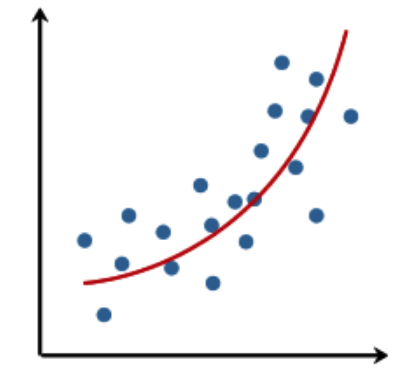
\includegraphics[width=0.9\linewidth]{figures-bias-var-tradeoff/non_linear_regression.png}
\end{figure}
$$\phi(x) = [1, x, x^2]$$
\end{minipage}

\end{frame}


\begin{frame}{Overfitting}
  \begin{figure}
    \centering
    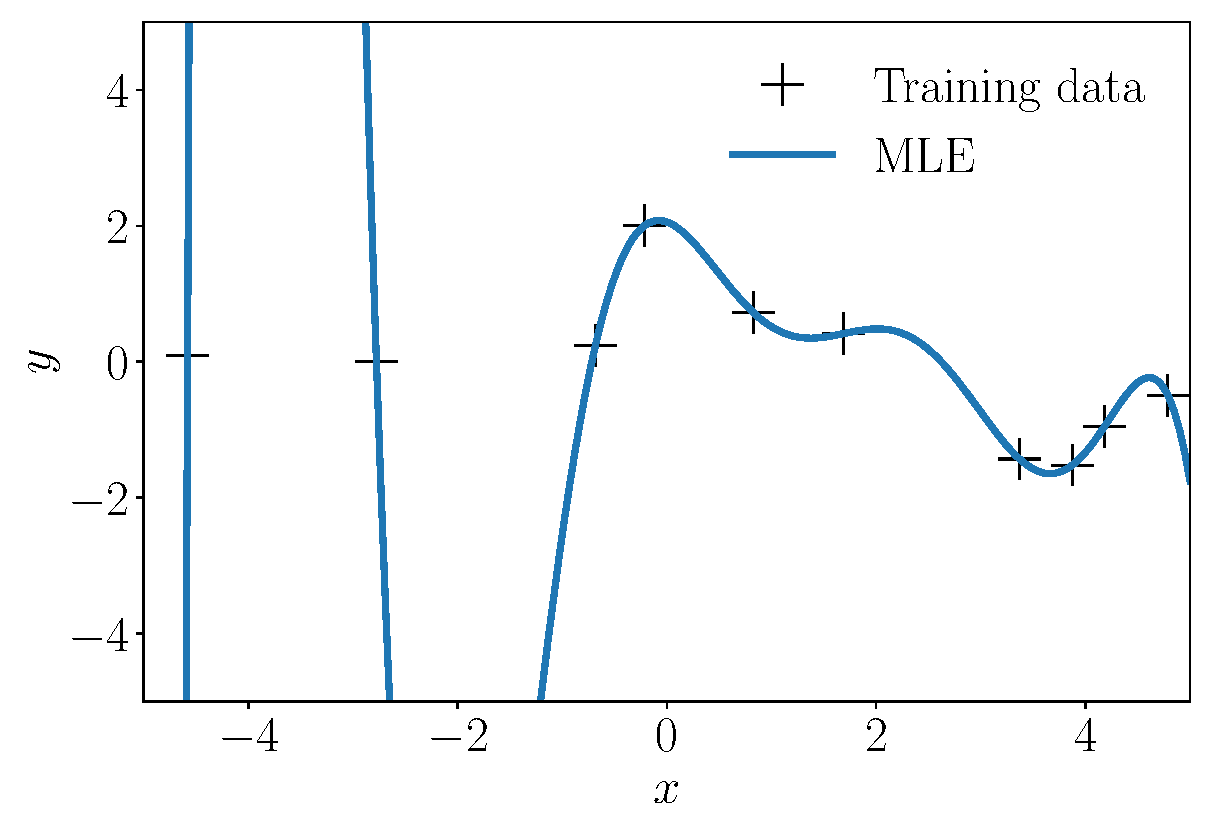
\includegraphics[width = 0.6\hsize]{./figures-bias-var-tradeoff/demo_regression_mle_10.pdf}
  \end{figure}
\begin{equation}
\phi(x) = [1\,\, x\,\, x^2\,\, x^3, \dots]^{\top}
\end{equation}
When the model is too flexible, risk of overfitting!
\end{frame}


\begin{frame}{Overfitting}

To help avoid overfitting:
\begin{itemize}
	\item Choose model with the right complexity (using validation data)
	\item \alert{Regularise the model} (this lecture)
		\begin{itemize}
		\item There's a bias-variance tradeoff here!
		\end{itemize}
\end{itemize}

\end{frame}

\begin{frame}
\frametitle{Regression with non-linear features}
Fitting regression model with a \emph{regulariser}:
$$L(\mparam) = \frac{1}{2 \sigma^2} \sum_{n} (f(\x_n, \mparam ) - y_n)^2 + \frac{\lambda}{2} || \mparam ||_2^2$$
\begin{itemize}
	\item \alert{Write $\Phi = [\phi(\x_1), ..., \phi(\x_N)]^\top \in \mathbb{R}^{N \times p}$}:
	$$\mparam^*_R = \argmin_{\mparam \in \Theta} \frac{1}{2 \sigma^2} || \y - \textcolor{red}{\Phi} \mparam ||_2^2  + \frac{\lambda}{2} ||\mparam||_2^2$$
	\item Optimal solution for $\mparam$:
	$$\mparam^*_R = (\sigma^2 \lambda \mathbf{I} + \textcolor{red}{ \Phi^\top \Phi })^{-1} \textcolor{red}{\Phi^\top} \y$$
\end{itemize}

\end{frame}


%%%%%%%%%

\begin{frame}
\frametitle{Intuition behind the regulariser}

Regression with polynomial functions as an example:
$$f(\x, \mparam) = \sum_{i=1}^p \theta_i \x^{i-1}$$

\begin{minipage}{0.45\linewidth}
\begin{figure}
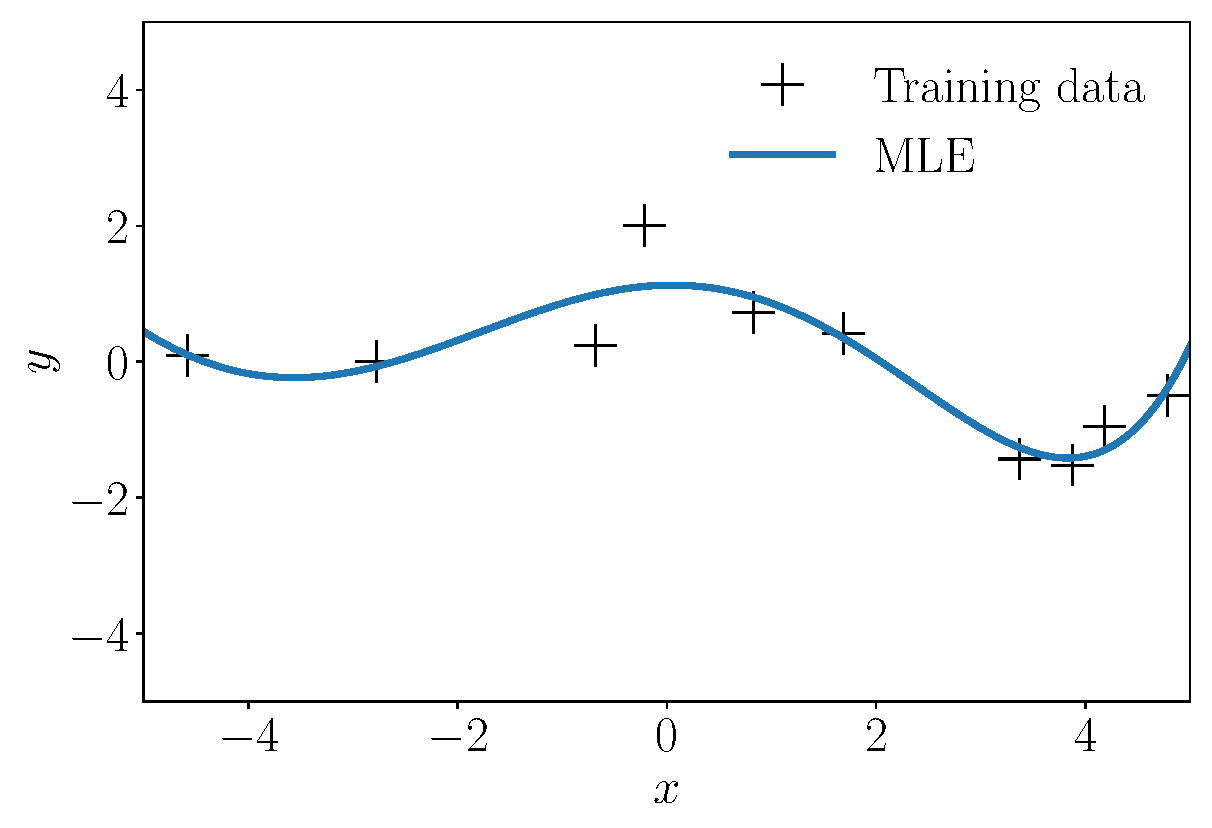
\includegraphics[width=0.9\linewidth]{figures-bias-var-tradeoff/demo_regression_mle_5.pdf}
\end{figure}
\end{minipage}
\hfill
\begin{minipage}{0.45\linewidth}
\begin{figure}
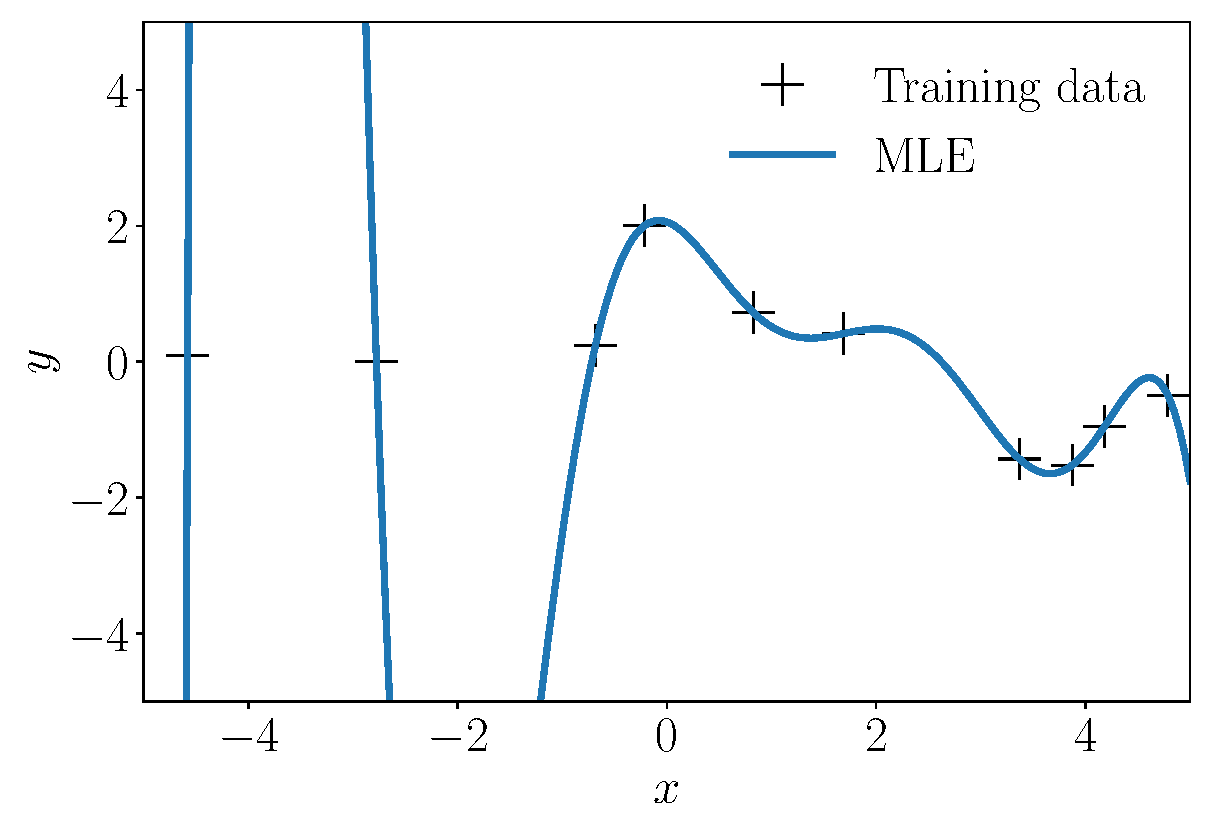
\includegraphics[width=0.9\linewidth]{figures-bias-var-tradeoff/demo_regression_mle_10.pdf}
\end{figure}
\end{minipage}
%


Several solutions fit the training data almost equally well.

$\Rightarrow$ How to choose a model?

\end{frame}


\begin{frame}
\frametitle{Intuition behind the regulariser}

Regression with polynomial functions as an example:
$$f(\x, \mparam) = \sum_{i=1}^p \theta_i \x^{i-1}$$

The $\ell_2$ regulariser used in ridge regression:
$$R(\mparam) = || \mparam ||_2^2 = \sum_{i=1}^p \mparam_i^2$$ 
\begin{itemize}
\item shrinks elements of $\mparam$ to zero \pause
\item if $\theta_i = 0$, then feature $\x^{i-1}$ is not in use \\ $\Rightarrow$ simpler model!
\item Ridge regression balances between data fit and model simplicity
\end{itemize}

\end{frame}

\begin{frame}
\frametitle{Intuition behind the regulariser}

Potential questions on using regularisers:
\begin{itemize}
	\item Do we obtain the ground truth parameters?
	\item Why regularised models can sometimes better fit the data (in terms of test error)?
\end{itemize}

To answer these: study Bias-variance tradeoff

\end{frame}


%%%%%%%%%% bias variance trade off %%%%%%%

\begin{frame}{Bias-variance tradeoff}

The general concept of Bias-variance tradeoff:
\begin{itemize}
	\item Suppose there is an unknown quantity $x_0$ that we like to estimate; 
	\item Assume we have a \emph{stochastic estimator} $X$ for $x_0$;
	\item Calculating the expected $\ell_2$ error:
	$$\mathbb{E}[ || X - x_0 ||_2^2] = \underbrace{|| \mathbb{E}[X] - x_0 ||_2^2}_{bias^2} + \underbrace{\tr[\mathbb{V}[X]]}_{variance}$$
	\begin{itemize}
		\item \emph{Unbiased} estimator: $bias = 0 \quad \Rightarrow \quad \mathbb{E}[X] = x_0$ 
		\item \emph{Low variance} estimator: variance is small
	\end{itemize}
\end{itemize}

\end{frame}


\begin{frame}{Bias-variance tradeoff}
Visualising Bias-variance trade-off:
\vspace{1em}

\begin{minipage}{0.4\linewidth}
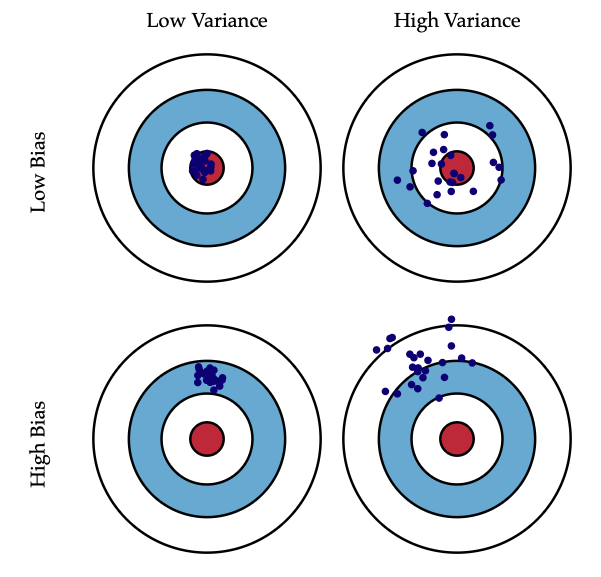
\includegraphics[width=1\linewidth]{figures-bias-var-tradeoff/bias_variance_vis.png}
\end{minipage}
\hfill
\begin{minipage}{0.55\linewidth}
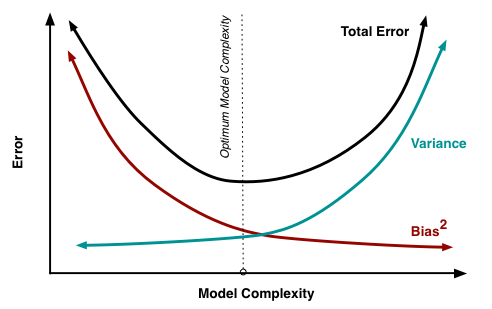
\includegraphics[width=1\linewidth]{figures-bias-var-tradeoff/biasvariance.png}
\end{minipage}

\hfill \tiny{Figures from \url{http://scott.fortmann-roe.com/docs/BiasVariance.html}}
\end{frame}

%%%%%%% regression example %%%%%

\begin{frame}
\frametitle{Bias-variance tradeoff in regression}

Fact for Ridge regression (linear regression + $\ell_2$ regulariser):

Ridge regression returns estimator of $\mparam$ which 
\begin{itemize}
\item is \emph{biased} (when $\lambda > 0$, unbiased only when $\lambda = 0$)
\item has \emph{smaller variance} than the MLE solution
\end{itemize}

With good choices of $\lambda > 0$, \alert{the (expected) test error can be reduced}.

\end{frame}


\begin{frame}{Bias-variance tradeoff in regression}
How bias-variance tradeoff is relevant to overfitting:

\alert{Expected} prediction error for $\mparam^* = \mparam^*(\mathcal{D})$ over $\mathcal{D} \sim \pi^N$:
\begin{equation*}
\begin{aligned}
error_{pred}(\mparam^*) &= \mathbb{E}_{\data \sim \pi^N} [ \mathbb{E}_{(\x_{test}, y_{test}) \sim \pi}[|| y_{test} - f(\x_{test}, \mparam^*(\data)) ||_2^2] ] \\
&= \mathbb{E}_{\x_{test}} [\phi(\x_{test})^{\top} \textcolor{red}{ Error(\mparam^*)} \phi(\x_{test})] + \sigma^2 \\
\end{aligned}
\end{equation*} 

\begin{equation*}
\begin{aligned}
Error(\mparam^*) &= \mathbb{E}_{\data \sim \pi^N}[ ( \mparam^*(\data) - \mparam_0 ) (\mparam^*(\data) - \mparam_0)^\top ] \\
&:=  \Bb(\mparam^*) \Bb(\mparam^*)^\top + \BV(\mparam^*)
\end{aligned}
\end{equation*}

\begin{equation*}
\begin{aligned}
\text{bias:} \quad & \Bb(\mparam^*) = \mathbb{E}_{\data \sim \pi^N}[\mparam^*(\data)] - \mparam_0 \\
\text{variance:} \quad & \BV(\mparam^*) = \mathbb{V}_{\data \sim \pi^N}[\mparam^*(\data)]
\end{aligned}
\end{equation*}

\end{frame}


\begin{frame}{Bias-variance tradeoff in regression}
How bias-variance tradeoff is relevant to overfitting:

\alert{Expected} prediction error for $\mparam^* = \mparam^*(\mathcal{D})$ over $\mathcal{D} \sim \pi^N$:
\begin{equation*}
\begin{aligned}
error_{pred}(\mparam^*) &= \mathbb{E}_{\data \sim \pi^N} [ \mathbb{E}_{(\x_{test}, y_{test}) \sim \pi}[|| y_{test} - f(\x_{test}, \mparam^*(\data)) ||_2^2] ] \\
&= \mathbb{E}_{\x_{test}} [\phi(\x_{test})^{\top} \textcolor{red}{ Error(\mparam^*)} \phi(\x_{test})] + \sigma^2 \\
\end{aligned}
\end{equation*} 
%
\begin{equation*}
Error(\mparam^*) = \Bb(\mparam^*) \Bb(\mparam^*)^\top + \BV(\mparam^*)
\end{equation*}

\pause


\vspace{1em}
If we have two estimators $\mparam_1$, $\mparam_2$ based on $\mathcal{D} \sim \pi^N$:
\begin{equation*}
Error(\mparam_1) \preceq Error(\mparam_2) \quad \Rightarrow \quad error_{pred}(\mparam_1) \leq error_{pred}(\mparam_2)
\end{equation*} 
\vspace{-2em}
\begin{itemize}
\item Smaller estimation error $\Rightarrow$ smaller prediction error
\item Depends on bias-variance trade-off
\end{itemize}

\end{frame}


\begin{frame}{Linear regression returns an unbiased estimator}
Reminder for solving linear/ridge regression:
\begin{itemize}
	\item Write $\Phi = [\phi(\x_1), ..., \phi(\x_N)]^\top \in \mathbb{R}^{N \times p}$:
	$$\mparam^* = \argmin_{\mparam \in \Theta} \frac{1}{2 \sigma^2} || \y - \Phi \mparam ||_2^2  + \frac{\lambda}{2} ||\mparam||_2^2$$
	\item Optimal solution for $\mparam$ in ridge regression:
	$$\mparam^*_R = (\sigma^2 \lambda \mathbf{I} + \Phi^\top \Phi )^{-1} \Phi^\top \y$$
	\item Optimal solution for $\mparam$ in linear regression ($\lambda = 0$):
	$$\mparam^*_L = (\Phi^\top \Phi )^{-1} \Phi^\top \y$$
\end{itemize}

\end{frame}

\begin{frame}{Linear regression returns an unbiased estimator}
Optimal solution for linear regression: $\mparam^*_L = (\Phi^\top \Phi )^{-1} \Phi^\top \y$

\begin{itemize}
\item Assuming no model error:
$$\y = \Phi \mparam_0 + \bm{\epsilon}, \quad \bm{\epsilon} = [\epsilon_1, ..., \epsilon_N]^\top, \quad \epsilon_n \sim \mathcal{N}(0, \sigma^2)$$
\item Leading to optimal solution as:
$\mparam^*_L = (\Phi^\top \Phi )^{-1} \Phi^\top (\Phi \mparam_0 + \bm{\epsilon})$
\item \alert{Unbiased estimator}:
\begin{equation*}
\begin{aligned}
\mathbb{E}_{\data \sim \pi^N}[\mparam^*_L(\data)] &= \mathbb{E}_{\data \sim \pi^N}[(\Phi^\top \Phi )^{-1} \Phi^\top (\Phi \mparam_0 + \bm{\epsilon})] 
= \mparam_0
\end{aligned}
\end{equation*}
\end{itemize}

\end{frame}


\begin{frame}{Ridge regression returns a biased estimator}

The ridge regression estimator: $\mparam^*_R = (\sigma^2 \lambda \mathbf{I} + \Phi^\top \Phi )^{-1} \Phi^\top (\Phi \mparam_0 + \bm{\epsilon})$

\begin{itemize}
\item Compute the mean of $\mparam^*_R$ for $\data \sim \pi^N$: 
\begin{equation*}
\mathbb{E}_{\data \sim \pi^N}[\mparam^*_R(\data)] = ( \sigma^2 \lambda \mathbf{I} + \Phi^\top \Phi )^{-1} \Phi^\top \Phi \mparam_0
\end{equation*}
$\Rightarrow$ Ridge regression returns a \alert{biased estimator} \pause

\item Compute the covariance matrix of $\mparam^*_R$ for $\data \sim \pi^N$:
\begin{equation*}
\begin{aligned}
\mathbb{V}_{\data \sim \pi^N}[\mparam^*_R(\data)] &= \mathbb{V}_{\data \sim \pi^N}[(\sigma^2 \lambda \mathbf{I} + \Phi^\top \Phi )^{-1} \Phi^\top (\Phi \mparam_0 + \bm{\epsilon})] \\
&=\mathbb{V}_{\data \sim \pi^N}[(\sigma^2 \lambda \mathbf{I} + \Phi^\top \Phi )^{-1} \Phi^\top \bm{\epsilon}] \\
&= \sigma^{2} (\sigma^2 \lambda \mathbf{I} + \Phi^\top \Phi )^{-1} \Phi^\top \Phi (\sigma^2 \lambda \mathbf{I} + \Phi^\top \Phi )^{-1} \\
\end{aligned}
\end{equation*}

\end{itemize}

\end{frame}


\begin{frame}{Ridge regression returns a biased estimator}

Bias of ridge regression estimator ($\lambda > 0$):
\begin{equation*}
\begin{aligned}
\Bb(\lambda) := \mathbb{E}_{\data \sim \pi^N}[\mparam^*_R(\data)] - \mparam_0 &= ( \sigma^2 \lambda \mathbf{I} + \Phi^\top \Phi )^{-1} \Phi^\top \Phi \mparam_0 - \mparam_0 \\
&= -\sigma^2 \lambda ( \sigma^2 \lambda \mathbf{I} + \Phi^\top \Phi )^{-1} \mparam_0
\end{aligned}
\end{equation*}

Bias of linear regression estimator ($\lambda = 0$): 
$$\Bb(0) = \bm{0}$$ \pause

Variance of ridge regression estimator ($\lambda > 0$): 
\begin{equation*}
\begin{aligned}
\BV(\lambda) &:= \sigma^2 (\sigma^2 \lambda \mathbf{I} + \Phi^\top \Phi )^{-1} \Phi^\top \Phi (\sigma^2 \lambda \mathbf{I} + \Phi^\top \Phi )^{-1}
\end{aligned}
\end{equation*}


Variance of linear regression estimator ($\lambda = 0$): 
$$\BV(0) = \sigma^2 (\Phi^\top \Phi )^{-1}$$

\end{frame}


\begin{frame}{Ridge regression can perform better in prediction}

\alert{Expected} prediction error of ridge regression ($\lambda > 0$):
\begin{equation*}
\begin{aligned}
error_{pred}(\mparam^*_R) &= \mathbb{E}_{\x_{test}} [\phi(\x_{test})^{\top} \textcolor{red}{ Error(\mparam_R^*) } \phi(\x_{test})] + \sigma^2 \\
Error(\mparam_R^*) &= \Bb(\lambda) \Bb(\lambda)^{\top} + \BV(\lambda)
\end{aligned}
\end{equation*}

\alert{Expected} prediction error of linear regression ($\lambda = 0$):
\begin{equation*}
\begin{aligned}
error_{pred}(\mparam^*_L) &= \mathbb{E}_{\x_{test}} [\phi(\x_{test})^{\top} \textcolor{red}{ Error(\mparam_L^*) } \phi(\x_{test})] + \sigma^2 \\
Error(\mparam_L^*) &= \Bb(0) \Bb(0)^{\top} + \BV(0) \textcolor{red}{= \BV(0)}
\end{aligned}
\end{equation*} \pause

This means if there exists some $\lambda > 0$ such that: 
\begin{equation*}
\Bb(\lambda) \Bb(\lambda)^\top + \BV(\lambda) \preceq \BV(0) \quad \Rightarrow \quad error_{pred}(\mparam_R^*) \leq error_{pred}(\mparam_L^*)
\end{equation*}

\end{frame}

\begin{frame}{Ridge regression can perform better in prediction}

Derivations exercises in the exercise sheet: \\

\begin{itemize}
\item For $\lambda >0 $, we can show reduced variance:
	$$\BV(\lambda) - \BV(0) \preceq 0$$

\item We can choose e.g.~$0 \leq \lambda \leq \frac{2}{|| \mparam_0 ||_2^2}$ which leads to:
$$ \Bb(\lambda) \Bb(\lambda)^\top + \BV(\lambda) \preceq \BV(0) \quad \Rightarrow \quad error_{pred}(\mparam_R^*) \leq error_{pred}(\mparam_L^*) $$

\item[$\Rightarrow$] The smaller prediction error of $\mparam_R^*$ comes from \\ having \alert{smaller variance} in parameter estimate!

\item[$\Rightarrow$] $\lambda$ needs to be chosen carefully so that \emph{the bias is not too large}

\end{itemize}


\end{frame}

\begin{frame}
\frametitle{Bias-variance tradeoff in regression: Summary}
\begin{center}
Ridge regression can return estimator of $\mparam$ with \alert{smaller variance}.

\vspace{1em}
In such case the (expected) test error can be reduced.
\end{center}

\begin{itemize}
\item $\mparam^*_R$ is a biased estimator of $\mparam_0$ when $\lambda > 0$
\item There exists $\lambda$ such that 
\begin{itemize}
	\item Variance is smaller: $\BV(\lambda) \preceq \BV(0)$ 
	\item Bias is not too large
\end{itemize}
\item ... and it leads to $error_{pred}(\mparam^*_R) \leq error_{pred}(\mparam^*_L)$
\end{itemize}
\end{frame}

\begin{frame}{Bias-variance tradeoff}
Visualising Bias-variance trade-off:
\vspace{1em}

\begin{minipage}{0.4\linewidth}
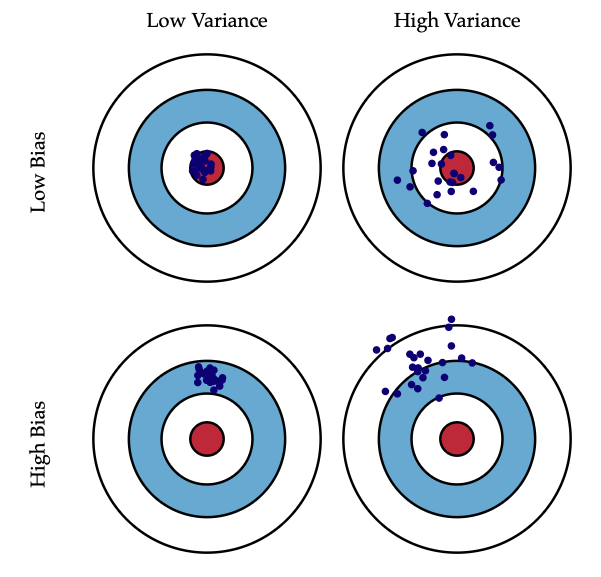
\includegraphics[width=1\linewidth]{figures-bias-var-tradeoff/bias_variance_vis.png}
\end{minipage}
\hfill
\begin{minipage}{0.55\linewidth}
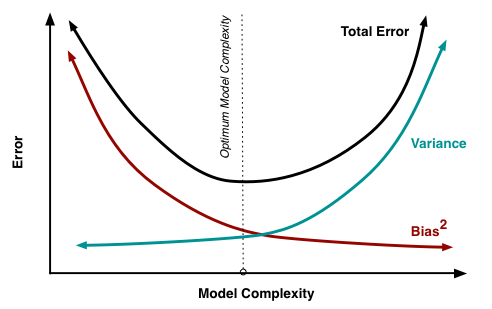
\includegraphics[width=1\linewidth]{figures-bias-var-tradeoff/biasvariance.png}
\end{minipage}

\hfill \tiny{Figures from \url{http://scott.fortmann-roe.com/docs/BiasVariance.html}}
\end{frame}


%%%%%%%%%%%%%%%%%%%%%%%%%%%%%%%%%%%%%%%%



\end{document}
%%% Local Variables: 
%%% mode: latex
%%% TeX-master: t
%%% End: 
